%
% File acl2017.tex
%
%% Based on the style files for ACL-2015, with some improvements
%%  taken from the NAACL-2016 style
%% Based on the style files for ACL-2014, which were, in turn,
%% based on ACL-2013, ACL-2012, ACL-2011, ACL-2010, ACL-IJCNLP-2009,
%% EACL-2009, IJCNLP-2008...
%% Based on the style files for EACL 2006 by 
%%e.agirre@ehu.es or Sergi.Balari@uab.es
%% and that of ACL 08 by Joakim Nivre and Noah Smith

\documentclass[11pt,a4paper]{article}
\usepackage{acl2017}
\usepackage{times}
\usepackage{latexsym}

% House Style
\usepackage{booktabs}

% Other Style
\usepackage{amsmath}
\usepackage{graphicx}
\usepackage{subfig}
\usepackage{algorithm}
\usepackage[noend]{algpseudocode}

\usepackage{url}

%\aclfinalcopy % Uncomment this line for the final submission
%\def\aclpaperid{***} %  Enter the acl Paper ID here

%\setlength\titlebox{5cm}
% You can expand the titlebox if you need extra space
% to show all the authors. Please do not make the titlebox
% smaller than 5cm (the original size); we will check this
% in the camera-ready version and ask you to change it back.

\newcommand\BibTeX{B{\sc ib}\TeX}

\title{Avoiding Coadaptation for Composition \\ when Exploring Tree Structures for Sequence Classification\Thanks{Thanks for the fish (obligatory {\em Hitchhiker's Guide} Reference)!}}

\author{Andrew Drozdov \\
  New York University \\
  Department of Computer Science \\
  {\tt apd283@nyu.edu} \\\And
  Samuel Bowman \\
  New York University \\
  Department of Data Science / Department of Linguistics \\
  {\tt bowman@nyu.edu} \\}

\date{}

\begin{document}
\maketitle
\begin{abstract}
  If it is true that some sequences have a tree-like optimal substructure that can
  be exploited for sequence labeling tasks, then this substructure (or a similar one) should be
  discoverable using Reinforcement Learning techniques.

  In this work, we present a task called LISTOPS which involves predicting the output
  of nested list operations. Since, SPINN performs much better than a comparable
  RNN, we determine that knowing that knowing the substructure of LISTOPS
  makes this a more feasible task. Nonetheless, when training
  SPINN's parsing component with the REINFORCE algorithm, it does not succeed
  to converge to a parsing strategy with a non-neglibible difference from a trivial
  parsing strategy. This is similar to what has been seen in related work, and we find this
  to be due to the following reasons:

1. There is a relationship between composition and parsing in SPINN. Composition is highly dependent on parsing.

2. Naively sampling random binary trees using transition based parsing does not uniformly sample over binary trees.

3. There is a lot of variance in this task, exacerbated by the label bias problem encountered in transition based parsing.

We address the first two issues by:

1. Using a soft wake sleep to interpolate between training the parser and the composition function, limiting the coadaptation between the two.

2. Sampling from a ``Catalan Pyramid'', ensuring a uniform distribution over binary trees.

Although do not treat the 3rd issue.

\end{abstract}

\section{Introduction}

TODO. Related work: SPINN + REINFORCE \cite{yogatama2016learning}; Inducing Parse Trees \cite{dyer2016rnng}

% Citations  \citet{bowman2016fast,yogatama2016learning,dyer2016rnng,rennie2016self,williams1992simple}

\section{SPINN + REINFORCE}

We use a slightly modified thin stack algorithm from \citet{bowman2016fast}
(pseudocode provided in Appendix A.\ref{rlloss}). It's
simple to add a method that trains the parser with the REINFORCE algorithm
\citep{williams1992simple}. REINFORCE approximates the gradient for non-differentiable
functions, and due to its high variance, it's necessary to subtract a baseline
from the reward. This difference (commonly called the advantage) has much less
variance and can be used to make more consistent gradient steps. In our case,
the reward is provided by the classification accuracy and we run our model in the
inference setting to baseline the reward \citep{rennie2016self}.

To illustrate why REINFORCE may be problematic in the context of SPINN, consider
a parser that returns strictly left branching trees (which turns out to be similar as
encoding a sequence in the forward direction with a Recurrent Neural Network -- RNN).
If you train a composition function with this fixated parser for a significant number
of examples, the composition function will coadapt to this forward sequential structure.
At this point, changing the behavior of the parser to return strictly right branching parse trees
(which is similar to encoding a sequence in the backward direction) will introduce examples
to the composition function that it has not seen previously, leading to noisy compositional
output, which will propogate noise to any downstream components of the model.

For these reasons, it's highly desirable to prevent coadaptation for two reasons:

\begin{enumerate}
\item
An unprepared compositional function propogates noise throughout the model, making
classification difficult and exploring non-trivial tree structures too costly.
\item
Models that attempt to explore will eventually follow a degenerate training regime and
fail at their semantic task.
\end{enumerate}

In the following section we detail a training strategy that prevents coadaptation and
improves the exploration of substructures, addressing these two problems.

\section{Soft Wake Sleep}

% Distribution Balanced Image
\begin{figure}[h]
\centering
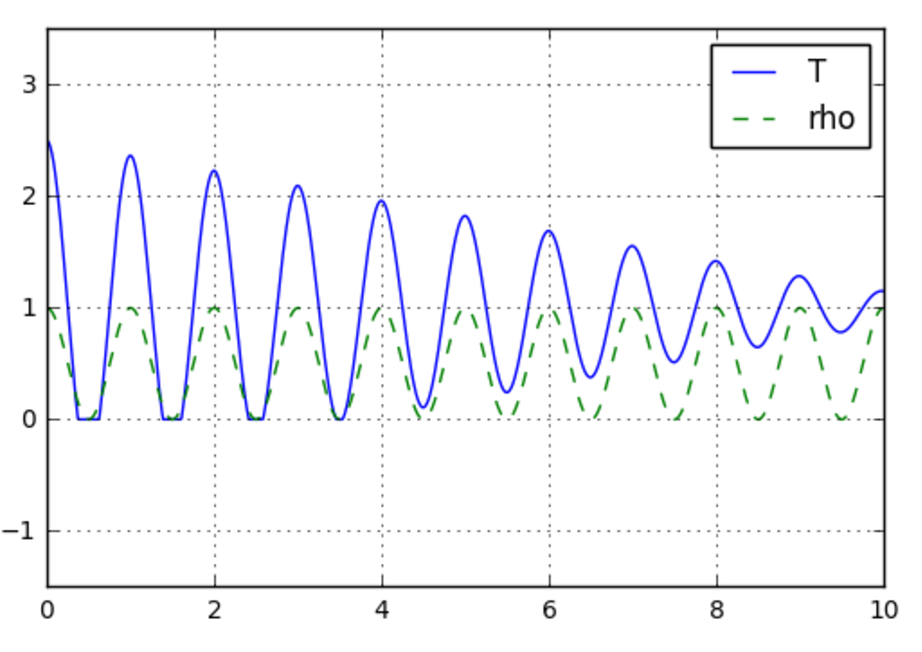
\includegraphics[width=7cm]{temperature_schedule}
\caption{The temperature T used to interpolate between greedy and random distributions when sampling transitions follows a strictly positive sinusoidal wave with annealed magnitude. The scale $\rho$ on the REINFORCE loss follows a similar schedule but is not annealed.}
\end{figure}

By interpolating between training the parser and the composition function, we apply
temperature to the softmax layer of the transition network defined by an annealed
sinusoidal schedule. We apply a similar temperature to scale the loss of the transition
network. The combination of these two actions searches randomly over all relevant binary
trees, teaching the parser to replicate only useful trees in the future and the composition
function to exhibit reasonable behavior over many different recursive trees.

Adding temperature to the softmax is done by dividing the input of the softmax by a variable
$T$. The output of the softmax resembles a uniform distribution when $T\to\infty$.

\begin{align}
\sigma(\frac{\vec{x}}{T}) = \frac{e^{\frac{x}{T}}}{\Sigma_{\hat{x} \in \vec{x}} e^{\frac{\hat{x}}{T}}}
\end{align}

% Distribution Step/Catalan Image
% \begin{figure}[tbp]
%   \centering
%   \subfloat[Uniformly Random]{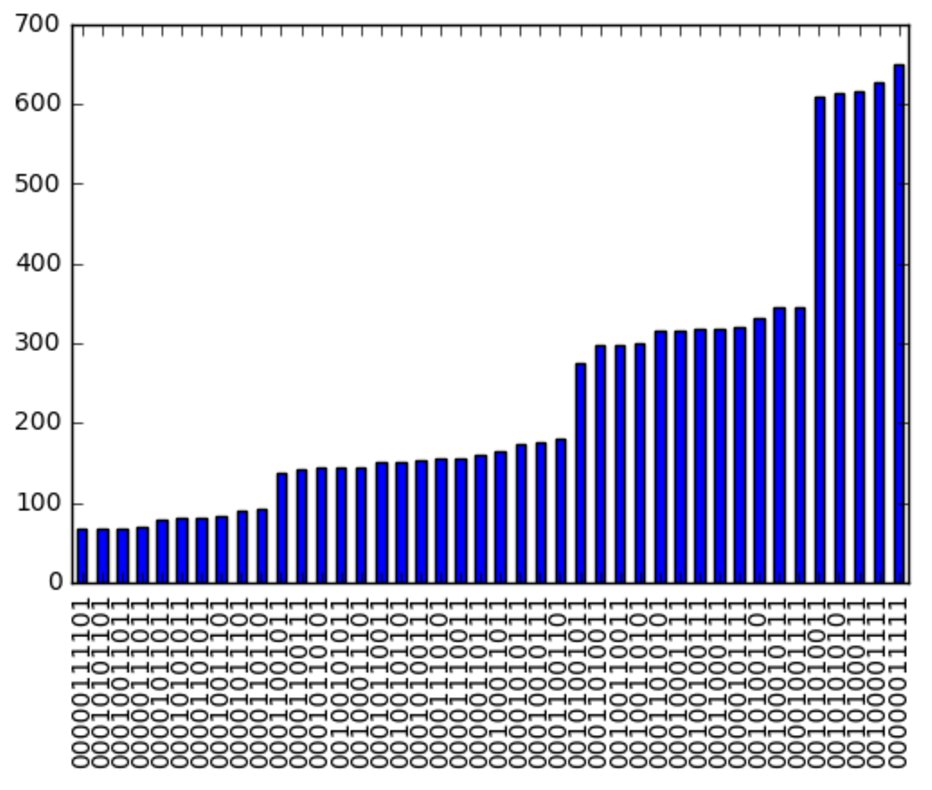
\includegraphics[width=0.2\textwidth]{distribution_step}\label{fig:f1}}
%   \hfill
%   \subfloat[Catalan Pyramid]{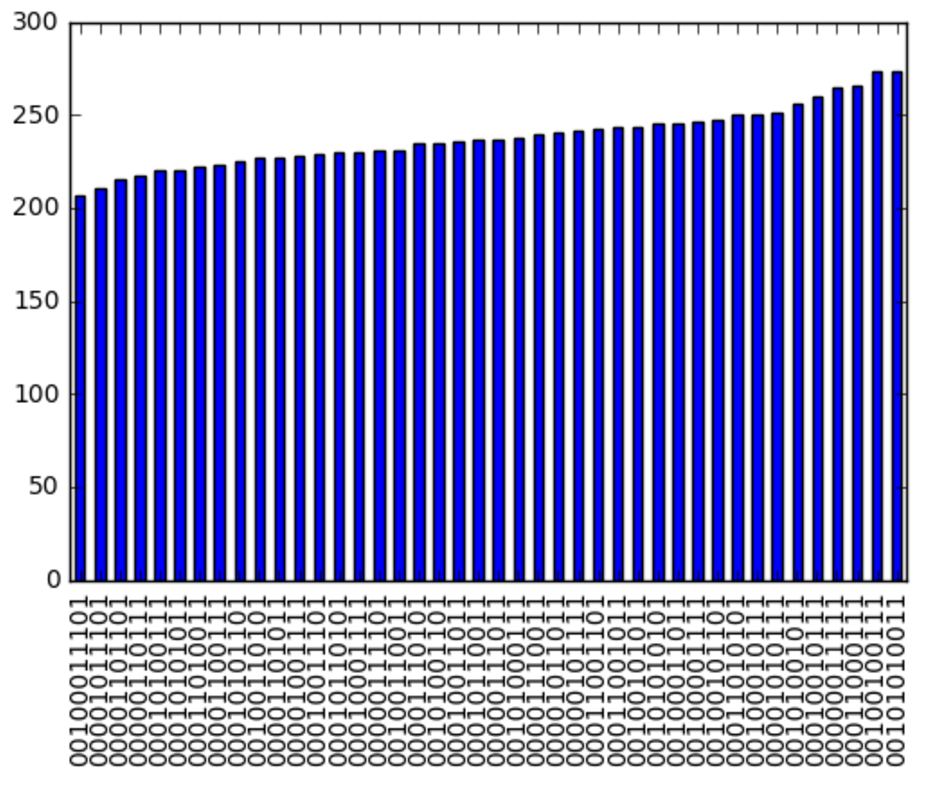
\includegraphics[width=0.2\textwidth]{distribution_balanced}\label{fig:f2}}
%   \caption{Frequency counts of randomly generated binary trees with N=6 leaves by using the a uniform distribution over Shift/Reduce transitions and the distribution from the Catalan Pyramid for Shift/Reduce transitions in sequence over 10k samples.}
% \end{figure}

\begin{figure}[h]
\centering
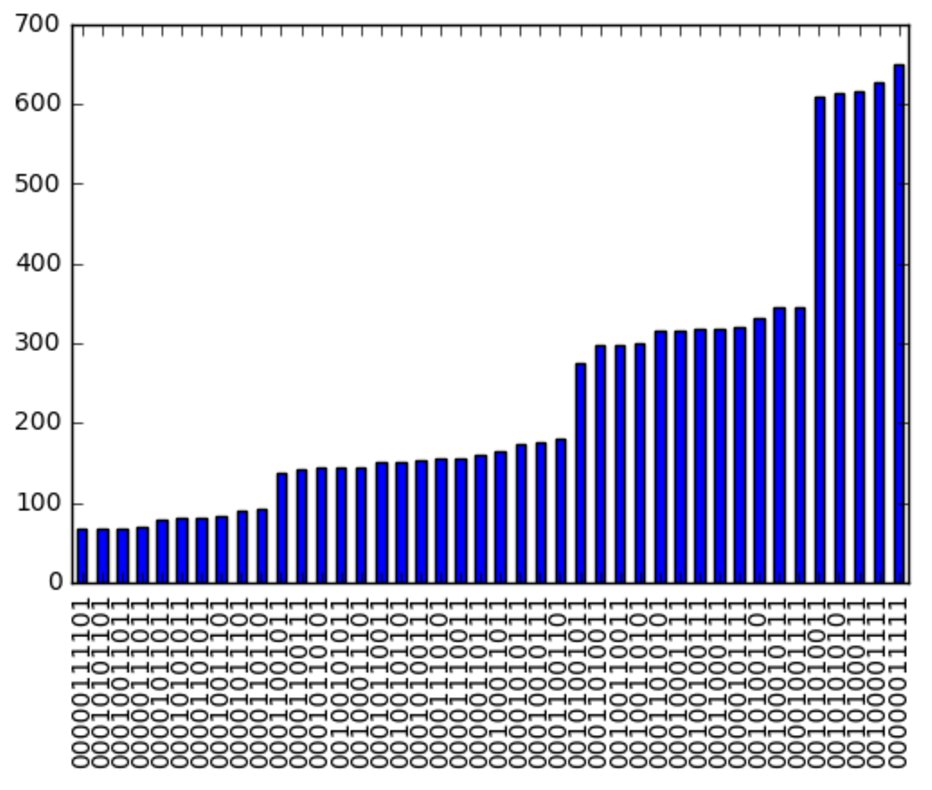
\includegraphics[width=7cm]{distribution_step}
\caption{Frequency counts of randomly generated binary trees with N=6 leaves by using the a uniform distribution over Shift/Reduce transitions and the distribution from the Catalan Pyramid for Shift/Reduce transitions in sequence over 10k samples.}
\label{fig:uniform}
\end{figure}

\begin{figure}[h]
\centering
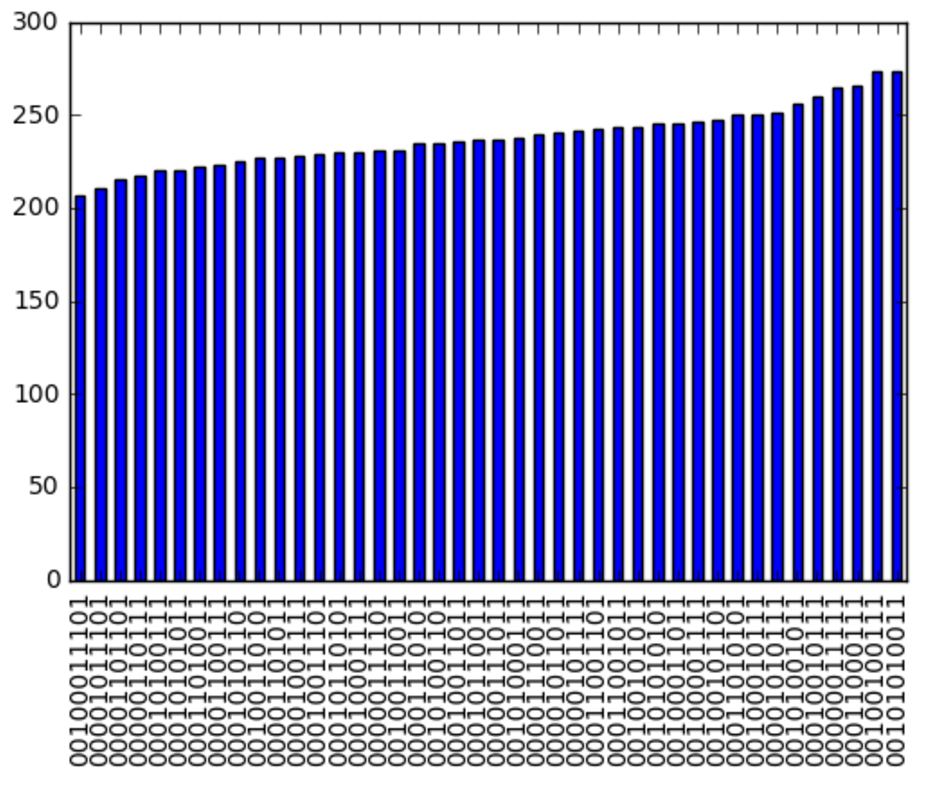
\includegraphics[width=7cm]{distribution_balanced}
\caption{Frequency counts of randomly generated binary trees with N=6 leaves by using the a uniform distribution over Shift/Reduce transitions and the distribution from the Catalan Pyramid for Shift/Reduce transitions in sequence over 10k samples.}
\label{fig:catalan}
\end{figure}

Iteratively uniformly sampling transitions does not lead to uniforming sampling over binary trees in Shift Reduce Transition Based Parsing. Rather, the distribution of trees resembles a step function as seen in Figure~\ref{fig:uniform}, which shows the frequency counts of binary trees over iterative random samples. To uniformly sample over binary trees, it's necessary to sample from a distribution representing the number of valid paths containing either Shift or Reduce as the next transition. A naive algorithm can come up with this distribution in exponential time by enumerating all possible trees of a given length, and filtering to relevant trees, but this approach is unusuable for trees with even a moderate number leaves. Fortunately, this distribution seems to have a closed form solution which can be recovered in linear time for any transition in any binary tree, and amortized constant time. We present the recursive algorithm in Figure~\ref{fig:catalan} and call the related distribution the Catalan Pyramid as each row contains fractions over the Catalan Numbers (which represent the count of binary trees with N leaves). A quick search did not turn up previous strategies for sampling uniformly over binary trees in transition based parsing.

The distribution from the Catalan Pyramid is not uniformly random at each time step, so the formula for temperature must be adjusted to take the proper distribution into account. Since temperature leads to a uniform distribution at its limit, it is a linear interpolation of the distribution based purely on the logits ($T = 1$) and the uniform distribution. We can recover the linear parameter directly to perform a similar interpolation between any distribution, including the one from the Catalan Pyramid.

\begin{align}
\sigma(\frac{\vec{x}}{T}) &= i \cdot \sigma(\vec{x}) + (1 - i) \cdot \sigma(0) \\
i &= \frac{\sigma(\frac{\vec{x}}{T}) - \sigma(0)}{\sigma(\vec{x})}
\end{align}

% Catalan Pyramid
\begin{table*}
\small
\centering
\begin{tabular}{|r|l|l|l|l|l|l|l|l|l|l|l|l|l|l|l|}
\hline & t=0 & 1 & 2 & 3 & 4 & 5 & 6 & 7 & 8 & 9 & 10 & 11 & 12 & 13 & 14 \\ \hline
r=0 & 1 & 1 & $\frac{297}{429}$ & $\frac{165}{297}$ & $\frac{75}{165}$ & $\frac{27}{75}$ & $\frac{7}{27}$ & $\frac{1}{7}$ &   &   &   &   &   &   &   \\
1 &   &   &   & 1 & $\frac{90}{132}$ & $\frac{48}{90}$ & $\frac{20}{48}$ & $\frac{6}{20}$ & $\frac{1}{6}$ &   &   &   &   &   &   \\
2 &   &   &   &   &   & 1 & $\frac{28}{42}$ & $\frac{14}{28}$ & $\frac{5}{14}$ & $\frac{1}{5}$ &   &   &   &   &   \\
3 &   &   &   &   &   &   &   & 1 & $\frac{9}{14}$ & $\frac{4}{9}$ & $\frac{1}{4}$ &   &   &   &   \\
4 &   &   &   &   &   &   &   &   &   & 1 & $\frac{3}{5}$ & $\frac{1}{3}$ &   &   &   \\
5 &   &   &   &   &   &   &   &   &   &   &   & 1 & $\frac{1}{2}$ &   &   \\
6 &   &   &   &   &   &   &   &   &   &   &   &   &   & 1 &   \\
\hline
\end{tabular}
\caption{Catalan Pyramid. Represents probability of predicting shift at timestep t given there have already been r reduces.}
\label{tab:catalan-pyramid}
\end{table*}

\section{Experiments}

TODO

\section{Discussion}

We succeed in consistently finding interesting parse trees, but are unable to find a benefit when it comes to predicting sequence lables nor recover a substructure that matches our expectations. We suspect that treating the 3rd issue could be key to future success with SPINN and REINFORCE.


\section*{Acknowledgments}

TODO

% include your own bib file like this:
%\bibliographystyle{acl}
%\bibliography{acl2017}
\bibliography{acl2017}
\bibliographystyle{acl_natbib}

\newpage

\appendix

\section{Algorithms}
\label{sec:algos}

\subsection{Supervised SPINN}
\label{sec:algos-spinn}

%%
% Supervised SPINN
\begin{algorithm}[H]
\caption{SPINN}\label{spinn}
\begin{algorithmic}[1]

\Function{SPINN}{sentences, Ts}
\State bufs := \{[$\vec{0}$] + s.reverse() $\vert$ s $\in$ sentences\}
\State stacks := \{[$\vec{0}$,$\vec{0}$] $\vert$ s $\in$ sentences\}
\State Ts$'$ := transitions.T
\For {ts $\in$ transitions}
 \State ts$'$ := \Call{BatchStep}{bufs, stacks, ts}
 \State Ts$'.push$(ts$'$)
 \EndFor
 \State \Return stacks[-1], Ts$'$
 \EndFunction

\Function{BatchStep}{bufs, stacks, ts}
\State inp := [bufs[-1], stacks[-1], stacks[-2]]
\State ts$'$ := $f^P$($f^T$(inp))
\State ts$'$ := \Call{Validate}{ts, ts$'$}
\State R, S := \Call{Distribute}{ts$'$, bufs, stacks}
\State \Call{Reduce}{R}; \Call{Shift}{S}
\State \Return ts$'$
\EndFunction

\Function{Distribute}{ts, bufs, stacks}
\State R, S $:= $ [], []
\For {t, S, Q $\in$ ts, bufs, stacks}
\If {$t = \text{REDUCE}$}
\State R$.push$(Q.pop(), S, Q)
\ElsIf {$t = \text{SHIFT}$}
\State right, left $:=$ S.pop(), S.pop()
\State S.$push$([left, right], S, Q)
\EndIf
\EndFor
\State \Return R, S
\EndFunction

\Function{Reduce}{R}
\State [lefts, rights], bufs, stacks := R.T
\State inp = [lefts, rights]
\State outp = split($f^C$(inp))
\For {o $\in$ outp, S $\in$ stacks}
\State S$.push$(o)
\EndFor
\EndFunction

\Function{Shift}{S}
\For {top, S, Q $\in$ S}
\State S$.push$(top)
\EndFor
\EndFunction

\end{algorithmic}
\end{algorithm}

\newpage

\subsection{Supervised Model}
\label{sec:algos-supervised}

%%
% Supervised Loss
\begin{algorithm}[H]
\caption{Supervised Model}\label{loss}
\begin{algorithmic}[1]

\Function{Model}{sentences, transitions, y}
\State Ts := transitions.T
\State outp, Ts$'$ := \Call{SPINN}{sentences, Ts}
\State y$'$ := $f^y$(outp)
\State Loss$_y$ := \Call{NLL}{y, y$'$}
\State Loss$_T$ := \Call{NLL}{Ts, Ts$'$}
\State \Return Loss$_y$, Loss$_T$
\EndFunction

\end{algorithmic}
\end{algorithm}

\subsection{Reinforce Model}
\label{sec:algos-rl}

% TODO:
% - Use distribution of transitions as input for reinforce
% - Use baseline

%%
% RL Loss
\begin{algorithm}[H]
\caption{Reinforce Model}\label{rlloss}
\begin{algorithmic}[1]

\Function{Model}{sentences, transitions, y}
\State Ts := transitions.T
\State outp, Ts$'$ := \Call{SPINN}{sentences, Ts}
\State y$'$ := $f^y$(outp)
\State Loss$_y$ := \Call{NLL}{y, y$'$}
\State Loss$_{RL}$ := \Call{Reinforce}{Ts$'$, Loss$_y$}
\State \Return Loss$_y$, Loss$_{RL}$
\EndFunction

\end{algorithmic}
\end{algorithm}

\newpage

\section{Catalan Pyramid}
\label{sec:catalan}

For a sequence with N tokens, N*2 - 1 transitions, and N - 1 reduce transitions, can build a so-called ``Catalan Pyramid'' (Table~\ref{tab:catalan-pyramid}) using these 6 rules:

\begin{enumerate}
\item
$row_{i,0,0} = 1$
\item
$row_{i,0,1} = i + 2$
\item
$row_{i,n_i-1,1} = Catalan(i + 2)$
\item
$row_{i,n_i-1,0} = row_{i,n_i-1,1} - row_{i-1,n_i-2,1}$
\item
$row_{i,j,0} = row_{i,j-1,1}$
\item
$row_{i,j,1} = row_{i,j,0} + row_{i-1,j,1}$
\end{enumerate}

These rules will build the non-zero fractions in each row of the table (0=numerator, 1=denominator), then padding the fractions as show with zeros will give you the probability of SHIFTing given that you are at timestep $t$ and have already REDUCEd $r$ times.

\end{document}
